\section{Specific Motions}

\subsection{Inverse Motions}
Next we explore specific cases of general motions.  
One type of specific motion is the {\bf inverse motion}, which allows
for a map from the current configuration back to the reference
configuration.

The map from $\vX$ to $\vx$ is one-to-one and invertible.  
We write the inverse map, from $\vx$ to $\vX$ as
\be
\vX = \vvarphi^{-1}(\vx,t) = \vvarphi^{-1}_t(\vx),
\label{eq:motion_inverse}
\ee
which maps the current configuration back to the reference 
configuration.


\subsection{Homogeneous Motions}
Another type of specific motion is a {\bf homogeneous motion}, which 
is linear with respect to the reference configuration $\vX$.  
Consider a Taylor series expansion of the motion about a point 
$\vX_0$,
\be
 \vvarphi(\vX) = \vvarphi(\vX_0) + \tFbold(\vX_0) \cdot 
 \{\vX - \vX_0\} + 
 \mbox{\small H.O.T.}
 \label{eq:Taylor_F}
\ee
When the deformation gradient $\tFbold$ is constant, thus the 
higher order terms ({\small H.O.T.}) are zero.  Thus, a homogeneous
motion requires that
\be
 \vvarphi(\vX) = \vvarphi(\vX_0) + \tFbold(\vX_0)
 \cdot \{\vX - \vX_0\} 
 \;\; \forall \;\; \{\vX\} \mbox{ and } \{\vX_0\} \in \cB.
 \label{eq:homogeneous_motion}
\ee

Homogeneous motions will consist of several subtypes of isochoric 
motions, such as translations, rotations, and special case stretches.  
Figure~\ref{fig:motion_family} illustrates the inheritance relationship
between motions and is explicated here:

\begin{Hremark}
\begin{itemize}
\item Homogeneous motions are a subset of general motions.
All homogeneous motions are motions, but not all motions are homogeneous
motions.
\item A homogeneous motion that is free from fixed points is a 
{\bf translation}.  
When a body translates, no part of the body is fixed in space.
\item A homogeneous motion that has a fixed point will 
be either a {\bf rotation} or a {\bf stretch}.  
\item Translations and rotations
are rigid body motions, which are in contrast to deformable body
motions, which occur as stretches.  
\item Stretches may be volume preserving (isochoric, $J=1$), or
non-isochoric ($J\neq1$).  All rigid body motions are isochoric.
\item Isochoric deformations often occur as shear, but there is one
special case deformation, absent of shear, that occurs when the volume
is preserved through expansion along one principal axis, and contraction 
along the other two principal axes.
\item The foregoing descriptions are explained in greater detail in
the following sections.
\end{itemize}
\end{Hremark}

%Next, we describe a set of motions that are linear with respect
%to the reference configuration $\vX$, which will be found to be
%translations, rotations, dilatational stretch, and isochoric stretch.

\begin{figure}[ht!]
  \begin{center}
    %\begin{overpic}[width=\textwidth,grid,tics=10,natwidth=620,natheight=564]{fig/motion_family.pdf}
    %\begin{overpic}[width=\textwidth,natwidth=620,natheight=564]{fig/motion_family.pdf}
    \begin{overpic}[width=\textwidth]{fig/motion_family.pdf}
      \put( 95, 21){$J$}
      \put(  5, 32){$J=1$}
      \put( 75.5, 45){$\frac{\Delta V}{V}$}
      \put( 16.9, 57.3){$\bar{\vu}$}
      \put( 35, 56.4){$\tRbold$}
      \put( 52.5, 56.4){$\tUbold \; \tvbold$}
    \end{overpic}
  \end{center}
  \caption{Taxonomy of general motions.}
  \label{fig:motion_family}
\end{figure}


%\subsection{Linear Motions}
%In this section, we consider the equation of a line
%\be
%y = f(x) =  m x + b,
%\ee
%as inspiration for writing (\ref{eq:displacement_vvarphi}) 
%as\footnote{
%For the time being, we will not be concerned with time $t$, so we
%eliminate it from our notation for the sake of brevity.}
%\be
%\vx = \vvarphi(\vX, t) = 
%\underbrace{\; \tMbold(t) \; \vX \;}_{\text{linear in $\vX$}} 
%\;\;\; + 
%\underbrace{\vb(t)}_{\text{constant in $\vX$}} 
%\stackrel{\mbox{\scriptsize set}}{=} \;\;\; \vX + \vu(\vX, t).
%\ee
%Then the displacement can be written as
%\begin{align}
% \vu(\vX, t) &= \tMbold(t) \vX + \vb(t) - \vX, \\
%          &= \left[\tMbold(t) - \vid\right] 
%          \vX + \vb(t). \label{eq:displacement_M}
%\end{align}
%In the following sections, we will be exploring the
%effect of ``slope'' $\tMbold$ and 
%``intercept'' $\vb$ on displacements $\vu$. 
%To explore some motions, we shall consider the two-dimensional
%body shown in Fig.~\ref{fig:configuration_reference}.  
%
%\begin{figure}[ht!]
%  \begin{center}
%    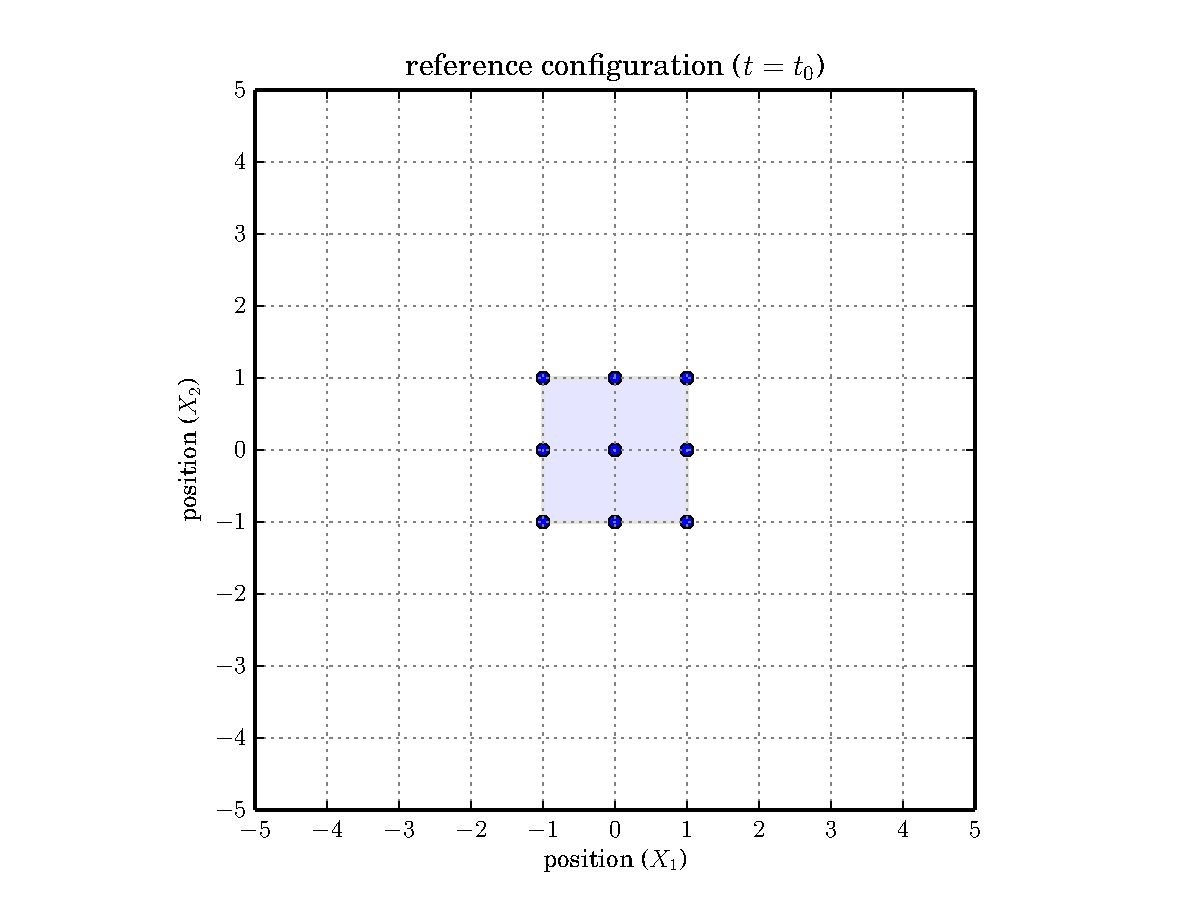
\includegraphics[width=\textwidth,natwidth=576,natheight=432]{fig/configuration_reference.pdf}
%    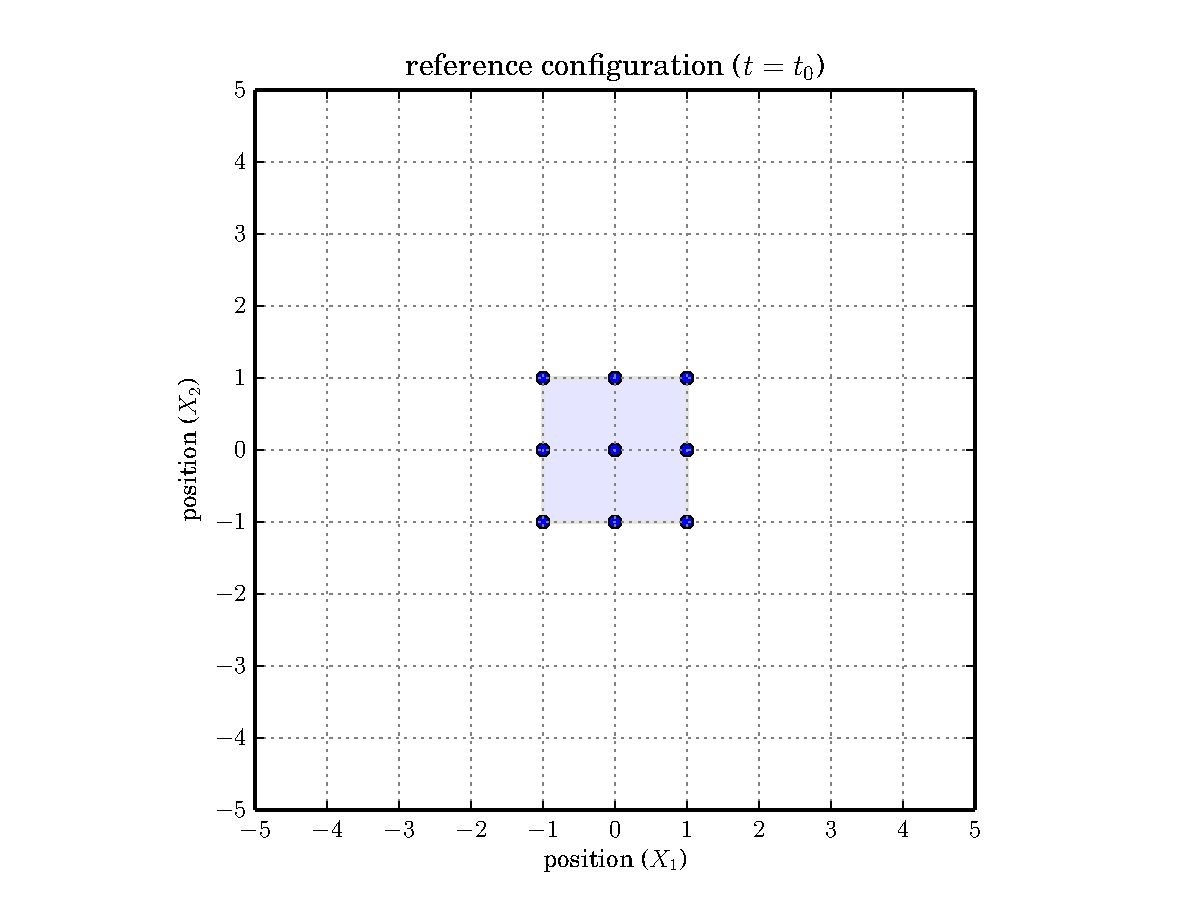
\includegraphics[width=\textwidth]{fig/configuration_reference.pdf}
%  \end{center}
%  \caption{Reference configuration of a body defined by particles
%  with $X_1 \in [-1, 1]$ and $X_2 \in [-1, 1]$.  With the 
%  continuum body is composed of an infinite number of particles, 
%  only nine particles are shown for the sake of simplicity.  Eight of
%  the nine particles shown are on the boundary of the body, and a 
%  single particle at the geometric center is the ninth particle.}
%  \label{fig:configuration_reference}
%\end{figure}
%
%The most elementary displacement is homogeneous, when 
%$\tMbold = \vid$ 
%and
%$\vb = \vzero$, then $\vu = \vzero$.
%In this case $\vvarphi = \vX$ and the motion is trivial (and
%uninteresting).  Nonetheless, this is a simple first case to consider.

\clearpage
\subsection{Translation}
\label{section:offset}
A translation is a homogeneous deformation of the form
\be
 \vvarphi(\vX) = \bar{\vu} + \vX.
\ee
This deformation occurs when the displacement 
$\vu(\vX, t$) is a constant 
$\bar{\vu}$, 
and thus not a function of 
reference position $\vX$ or time $t$.

%Next, consider $\vb \neq \vzero$, while
%retaining $\tMbold = \vid$.   
For the concrete example 
in Figure~(\ref{fig:configuration_current}), let 
$\bar{\vu} = \langle \bar{u}_1, \bar{u}_2 \rangle\transpose = 
\langle 3, 2 \rangle\transpose$.
In this case, we see the placement $\vvarphi$ moves right and up
on the page, relative to the reference configuration $\vX$, by 
an amount of 3 and 2, respectively.  
The reference configuration is shown in blue.  
The current configuration is shown in red.
\begin{figure}[htb]
  \begin{center}
    %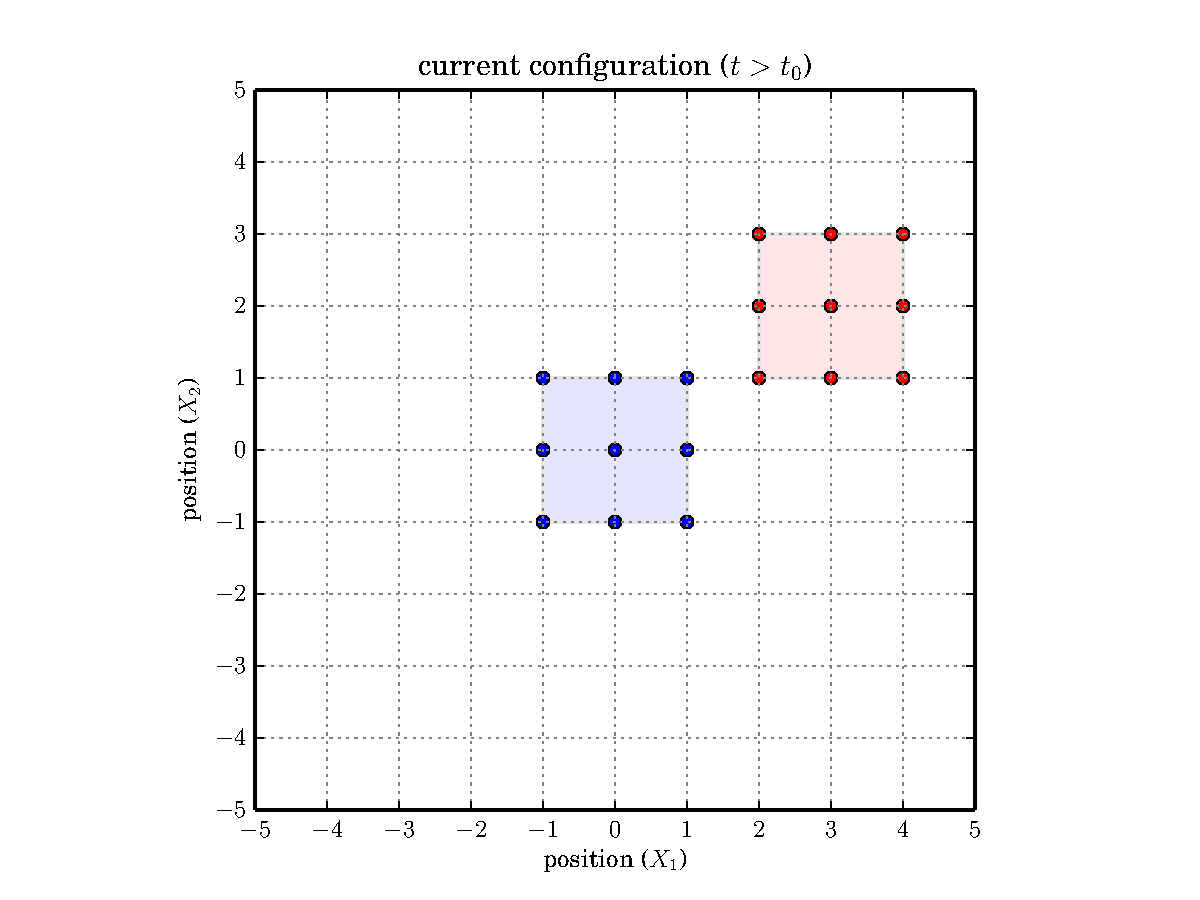
\includegraphics[width=0.8\textwidth,natwidth=576,natheight=432]{fig/configuration_current.pdf}
    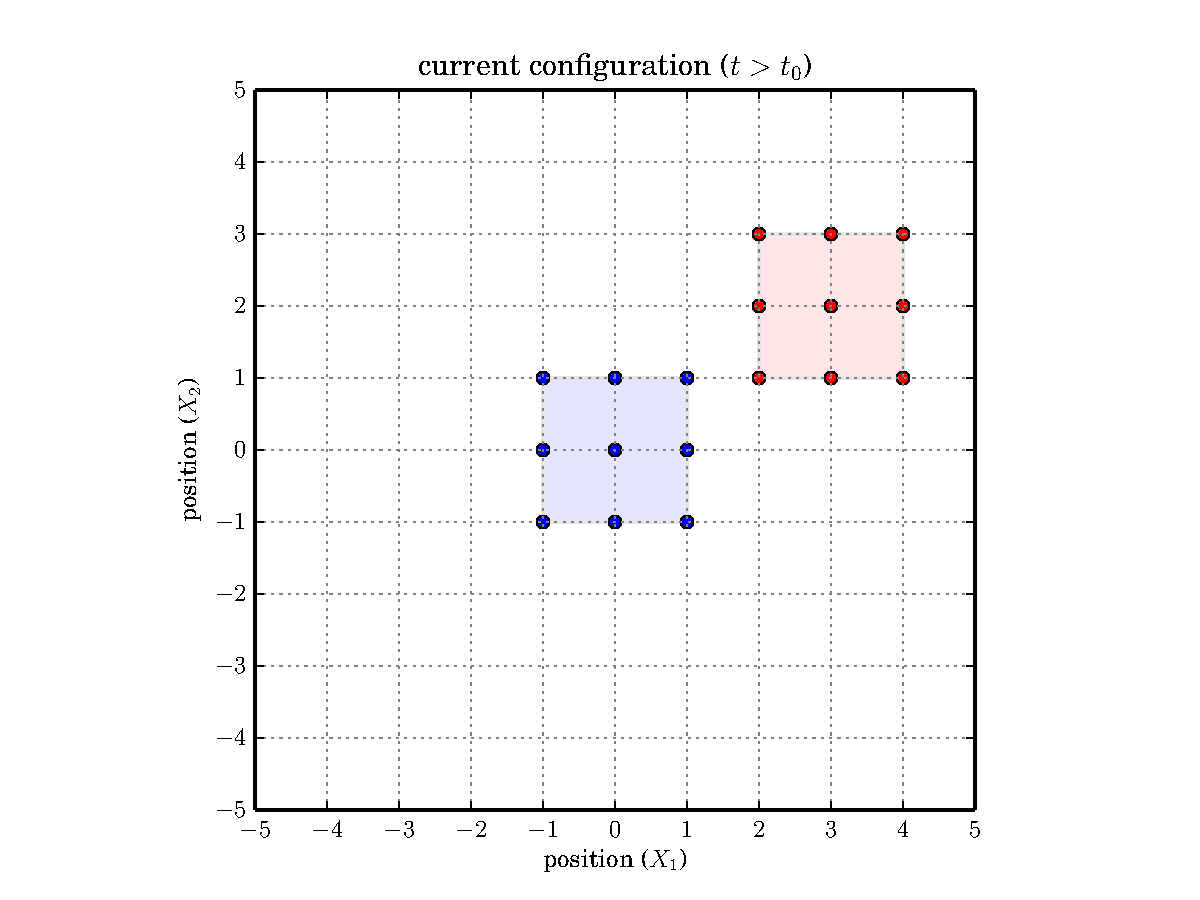
\includegraphics[width=0.8\textwidth]{fig/configuration_current.pdf}
  \end{center}
  \caption{Illustration of a translational motion.}
  \label{fig:configuration_current}
\end{figure}

\subsection{Fixed Point}
A fixed point deformation is a homogeneous deformation of the 
form
\be
 \vvarphi(\vX) = \vX_0 + \tFbold \cdot \{\vX - \vX_0\}.
\ee
The deformation is fixed in the sense that $\vvarphi(\vX_0) = \vX_0$.


\clearpage
\subsection{Rotation}
A rotation is a homogeneous deformation of the form
\be
 \vvarphi(\vX) = \vX_0 + \tRbold \cdot \{\vX - \vX_0\},
\ee
where the rotation occurs about the point $\vX_0$.

A rigid body motion, consisting of body translation and rotation, 
has the form
\be
 \vvarphi(\vX) = \bar{\vu} + \vX_0 + \tRbold \cdot \{\vX - \vX_0\}, 
\ee
where the translation is $\bar{\vu}$ and the rotation occurs around
point $\vX_0$.

To motivate rotations of deformable bodies, we start with two simpler
cases: general motion two {\em particles} instead of bodies, 
and general motion of {\em rigid} bodies instead of 
deformable bodies.  These two specific cases will then be building blocks
for the more general case of rotation of a deformable body, with 
and without stretch.

We first consider two particles, and 
describe absolute motion versus relative motion of particles.
Then, we connect two particles to create a two-particle body, and show
how a rigid body assumption leads to the absence of relative
translation between the particles of a body.  
While the absence of 
relative translation leads to the absence of absolute {\bf translation} between
two particles, remarkably, two particles can still move relative to
each other without violating the rigid body assumption and produce 
absolute translation through {\bf rotation} of the rigid body.

Finally, we connect these two ideas---translation of particles and rotation
of a rigid body---to describe the general case described as a particle
moving on a rigid body.  This formulation will then be further generalized
to describe motion composed of {\em both} rotation and stretch of a 
deformable body.

\subsubsection{Translation of Particles}
Consider two particles $P$ and $Q$ located in the in the 
inertial reference from $\cF$ and located with position vectors
$\vX_{P}$ and $\vX_{Q}$ from origin $O$.

For the time being, assume we know how particle $Q$ moves
in frame $\cF$ and how particle $P$ moves {\em relative} to 
particle $Q$.  Given these two knowns, we wish to construct 
an absolute relationship for how particle $P$ moves in the
inertial reference frame $\cF$.

To achieve this, 
we write the {\bf loop vector},
\be
\vX_{P} = \vX_{Q} + \vX_{P/Q}
\label{eq:loop_vector}
\ee
in the reference configuration, which stays that distance 
to point~$P$
from the origin~$O$
is equal to the 
distance 
to point~$Q$ 
from the origin~$O$ 
plus the distance 
to point~$P$ 
from point~$Q$.\footnote{This term, $\vX_{P/Q}$, is written in a 
way that is reminiscent of 
{\bf conditional probabilities}, that is ``the distance to 
point~$P$ {\em given} point~$Q$.}
Note, we could have written $\vX_P$ explicitly as $\vX_{P/O}$, but
drop the notation of the origin $O$ when it is used as the datum.
This relationship extend to the 
current configuration through the absolute and relative displacement
measures. The current placement of $P$,  
$\vx_{P}$, is the superposition  
of the current placement of $Q$ with the current placement of
$P$ {\em relative} to the current placement of $Q$. 
Explicitly,
\be
\vx_{P}(\vX, t) = \vX_{Q} + \vu_Q(\vX, t) + 
                  \vX_{P/Q} + \vu_{P/Q}(\vX, t).
\label{eq:loop_current}
\ee
The velocity of point $P$ is constructed by time-differentiating
(\ref{eq:loop_current}) to obtain
\be
\dot\vx_{P} = 
\frac{\partial \vu_Q}{\partial \vX_Q}
\cancelto{0}{\frac{\partial \vX_Q}{\partial t}} + 
\frac{\partial \vu_Q}{\partial t} 
\;\;+\;\;
\frac{\partial \vu_{P/Q}}{\partial \vX_{P/Q}}
{\frac{\partial \vX_Q}{\partial t}} +
\frac{\partial \vu_{P/Q}}{\partial t}.
\ee
Substituting (\ref{eq:loop_vector}) gives
\be
\dot\vx_{P} = 
\frac{\partial \vu_Q}{\partial \vX_Q}
\cancelto{0}{\frac{\partial \vX_Q}{\partial t}} + 
\frac{\partial \vu_Q}{\partial t} 
\;\;+\;\;
\frac{\partial \vu_{P/Q}}{\partial \vX_{P/Q}}
\left(
 \cancelto{0}{\frac{\partial \vX_P}{\partial t}} - 
 \cancelto{0}{\frac{\partial \vX_Q}{\partial t}}
\;\;\;\right)
+ 
\frac{\partial \vu_{P/Q}}{\partial t}.
\ee
Thus, the absolute velocity of point $P$ 
simply the absolute velocity of point $Q$ plus the 
relative velocity of point $P$ taken with respect to point $Q$,
\be
\vv_{P} = \vv_Q + \vv_{P/Q},
\ee
Similarly, for 
the accelerations,
\be
\va_{P} = \va_Q + \va_{P/Q}.
\ee
The canonical example of relative position, velocity, and acceleration
is that of a person, $P$, walking down the aisle of a passenger 
train $Q$.  The current position of the passenger in the inertial
reference $\vx_P$ is equal to the superposition of the 
current position of the train car in the inertial reference frame
$\vx_Q$ plus the position of the person {\em relative}
to the train car, $\vx_{P/Q}$.  This relationship, and the 
corresponding velocity and acceleration relationship, are 
stated explicitly as
\begin{align}
 \vx_P & = \vx_Q + \vx_{P/Q}, \\
 \vv_P & = \vv_Q + \vv_{P/Q}, \\
 \va_P & = \va_Q + \va_{P/Q}. 
\end{align}



%
\subsubsection{Rotation of a Rigid Body with Two Fixed Particles}
Next, we construct a rigid body by rigidly connecting particle 
$P$ and particle $Q$.  Thus, we have a body $\cB$ consisting of two 
particles.  Unlike particles, which have only three translation 
degrees of freedom, 
rigid bodies have six degrees of freedom: 
three translations and three rotations.

In the previous section, translation of particle $P$ 
required that either translation of particle $Q$,
or translation of particle $P$ {\em relative} to particle $Q$.
This last term, translation of particle $P$ relative to particle
$Q$, can be interpreted as a positive or negative {\bf stretch} 
between $P$ and $Q$ as motion from the reference configuration to the
current configuration occurs.

In this current section, we have constructed a rigid body out of
and between particles $P$ and $Q$.  Intuition then suggests 
positive or negative stretch between the two points can not occur, the
distance between particles $P$ and $Q$ in body $\cB$ is constant 
for all time.  

Remarkably, motion of particle $P$ can still occur not only as a consequence
of translations of particle $Q$, but also from rotations of body $\cB$
about an axis that contains $Q$.  In fact, because of superposition
of these two effects, even if particle $Q$ never moves, particle $P$ 
can move by virtue of rotations.

To come:  discussions on
$\ve{\omega}$, $\ve{\Omega}$, $\ve{\mathit{\Omega}}$, 
$\ve{\mathit{\omega}}$, 
$\widehat{\tWbold} = \tWbold_{\times}$, 
$\widehat{\twbold} = \twbold_{\times}$.

\begin{Hresult}
A special case of a motion $\vvarphi$ 
that is a rigid body motion has the form 
\be
  \vvarphi(\vX,t) = \tRbold(t) \vX + \vb(t)
  \;\;\Longleftrightarrow\;\;
  \varphi_i = \tR_{iJ} X_J + b_i.
  \label{eq:rigid_body_motion}
\ee
\end{Hresult}

\begin{Hresult}
The material velocity $\vV$ of the rigid body motion has the form
\be
  \vV(\vX,t) = \dot{\tRbold}(t) \vX + \dot{\vb}(t)
  \;\;\Longleftrightarrow\;\;
  V_I = \delta_{Ii} \dot{\tR}_{iJ} X_J + \delta_{Ii} \dot{b}_i.
  \label{eq:material_velocity}
\ee
\end{Hresult}

\begin{Hresult}
The material acceleration $\vA$ of the rigid body motion has the form
\be
  \vA(\vX,t) = \ddot{\tRbold}(t) \vX + \ddot{\vb}(t)
  \;\;\Longleftrightarrow\;\;
  A_I = \delta_{Ii} \ddot{\tR}_{iJ} X_J + \delta_{Ii} \ddot{b}_i.
  \label{eq:material_acceleration}
\ee
\end{Hresult}

It is more common to see the velocity and acceleration of the rigid
body expressed in the current configuration, as opposed to the reference 
configuration, as 
in (\ref{eq:material_velocity}) 
and (\ref{eq:material_acceleration}).




\begin{Hresult}
The current velocity $\vv$ of the rigid body motion has the form
\be
  \vv(\vx,t) = \vomega (t) \times 
  \left[ \;
  \vx - \vb(t)
  \; \right]
  + 
  \dot{\vb}(t)
  \;\;\Longleftrightarrow\;\;
  v_i = \epsilon_{ijk} \; \omega_j
  \left[ \;
  x_k - b_k
  \; \right]
  + 
  \dot{b}_i
  \label{eq:current_velocity}
\ee
\end{Hresult}

\begin{Hremark}
From time-to-time, and for
the sake of brevity, 
we avoid writing explicit dependence on time, $t$.
Thus, we write vector functions
simply as function of $\vX$ or $\vx$, and where dependence on $t$ 
is implied where appropriate.
\end{Hremark}

\begin{Hproof}
Rewrite rigid body motion (\ref{eq:rigid_body_motion})
in the current configuration $\vx$
\be
  \vx = \tRbold \; \vvarphi^{-1}(\vx) + \vb 
\ee
or
\be
  \vvarphi^{-1}(\vx) = 
  \tRbold^{-1} \left( \vx - \vb \right). 
\ee
Since $\tRbold^{-1} = \tRbold^T$, 
\be
  \vvarphi^{-1}(\vx) = 
  \tRbold(t)^T \left( \vx - \vb \right). 
  \label{eq:inverse_rigid_motion}
\ee
Write the velocity in the current configuration, 
$\vv(\vx,t)$, using (\ref{eq:material_velocity}) 
and use explicit time dependence on $t$ for clarity,
\be
\vv(\vx, t) = 
\vV(\vvarphi^{-1}(\vx, t), t) = 
\dot{\tRbold}(t) \; \vvarphi^{-1}(\vx, t) + \dot{\vb}(t).
\ee
Substitute (\ref{eq:inverse_rigid_motion}),
\be
\vv(\vx) = 
\underset{\left[\;\ve{\omega}\;\right]_{\times}}{\underbrace{\dot{\tRbold} \; \tRbold^T}}
\left( \vx - \vb \right) 
+ \dot{\vb}, 
\label{eq:velocity_current_penultimate}
\ee
where
\be
 \left[\;\ve{\omega}\;\right]_{\times} \vz = \vomega \times \vz = \dot{\tRbold} \; 
 \tRbold^T \; \vz,
 \label{eq:omega_hat}
\ee
for all vectors $\vz$.
With (\ref{eq:omega_hat}), 
(\ref{eq:velocity_current_penultimate}) can be written as
\be
\vv(\vx) = 
\vomega \times 
\left( \vx - \vb \right) 
+ \dot{\vb}, 
\ee
which is the result.
\end{Hproof}

\begin{Hresult}
The current acceleration $\va$ of the rigid body motion has the form
\be
  \va(\vx,t) = \valpha (t) \times 
  \left[ \;
  \vx - \vb(t)
  \; \right]
  + 
  \vomega (t) \times 
  \left( 
  \vomega (t) \times 
  \left[ \;
  \vx - \vb(t)
  \; \right]
  \right)
  + 
  \ddot{\vb}(t)
  \label{eq:current_acceleration}
\ee
\be
\;\;\Longleftrightarrow\;\;
  a_i = \epsilon_{ijk} \; \alpha_j
  \left[ \;
  x_k - b_k
  \; \right]
  + 
  \epsilon_{ijk} \; 
  \epsilon_{klm} \;
  \omega_j \;
  \omega_l \;
  \left[ \;
  x_m - b_m
  \; \right]
  +
  \ddot{b}_i
\ee
\end{Hresult}


\begin{Hproof}
Start with (\ref{eq:velocity_current_penultimate}) and differentiate
with respect to time, 
\be
\va(\vx, t)
= 
\frac{d}{dt}
\vv(\vx, t)
 = 
\frac{d}{dt}
\left(
\dot{\tRbold} \; \tRbold^T
\left( \vx - \vb \right) 
+ \dot{\vb}\right). 
\ee
Then expand,
\be
\va(\vx, t)
= 
\ddot{\tRbold} \; \tRbold^T
\left( \vx - \vb \right) 
+ 
\dot{\tRbold} \; \dot{\tRbold}^T
\left( \vx - \vb \right) 
+
\dot{\tRbold} \; \tRbold^T
\left( \dot{\vx} - \dot{\vb} \right) 
+
\ddot{\vb}. 
\label{eq:acceleration_current_penultimate}
\ee
The first two terms on the right-hand-side of
(\ref{eq:acceleration_current_penultimate}) 
can be combined and simplified to
\be
\left[
\ddot{\tRbold} \; \tRbold^T 
+ 
\dot{\tRbold} \; \dot{\tRbold}^T
\right] \; (\;\cdot\;)
= 
\frac{d}{dt}\;
\left[
\dot{\tRbold} \; \tRbold^T
\right]
\; (\;\cdot\;)
= 
\frac{d}{dt}\;[\;\vomega\;]_{\times}
\; (\;\cdot\;)
=
[\;\valpha \;]_{\times} \; (\;\cdot\;),
\ee
where $(\;\cdot\;)$ stands in for the $(\vx - \vb)$ vector.
The third term on the right-hand-side of 
(\ref{eq:acceleration_current_penultimate}), with
substitution of
(\ref{eq:velocity_current_penultimate}),
can be rewritten as
\be
\dot{\tRbold} \; \tRbold^T
\left( \dot{\vx} - \dot{\vb} \right) 
= 
\dot{\tRbold} \; \tRbold^T
\left(  
\dot{\tRbold} \; \tRbold^T
\left(\vx - \vb \right)
\right) 
= 
\vomega \times
\left(
\vomega \times (\;\cdot\;)
\right).
\ee
Combining these successive terms gives
\be
  \va(\vx) = \valpha  \times 
  \left( \;
  \vx - \vb
  \; \right)
  + 
  \vomega \times 
  \left( 
  \; \vomega \times 
  \left( \;
  \vx - \vb
  \; \right)
  \right)
  + 
  \ddot{\vb},
\ee
which is the result.
\end{Hproof}

\begin{Hresult}
{\bf Rodrigues Rotation Formula.}  The rotation of the position vector 
$\vr^{QP}$ into the position vector $\vr^{Qp}$ by rotation $\theta \vnhat$
is given by
\be
\vr^{Qp} = (1 - \cos \theta) \; (\vr^{QP} \cdot \vnhat) \; \vnhat + 
\cos \theta \; \vr^{QP} + \sin \theta \; (\vnhat \times \vr^{QP})
\ee
\end{Hresult}

\begin{Hproof}
Let the shorthand notation $\va = \vr^{QP}$ and $\vb = \vr^{Qp}$ be used
such that the rotation $\theta \vnhat$ rotates vector $\va$ into vector $\vb$. 
Furthermore, let the vectors $\va$ and $\vb$ 
be decomposed into the sum of two 
subspace vectors, 
which are parallel and perpendicular to the $\vnhat$ vector, such that 
\begin{align}
\va & = \va_{\|} + \va_{\perp} \;\; \Longleftrightarrow \;\; 
\va_{\perp} = \va - \va_{\|} \;\; \mbox{ and }  \;\;
\va_{\|} = (\va \cdot \vnhat) \; \vnhat, \\
\vb & = \vb_{\|} + \vb_{\perp} \;\; \Longleftrightarrow \;\; 
\vb_{\perp} = \vb - \vb_{\|} \;\; \mbox{ and }  \;\;
\vb_{\|} = (\vb \cdot \vnhat) \; \vnhat.
\end{align}
From inspection of the rotation plane perpendicular to $\vnhat$, as shown
in Fig.~\ref{fig:rigid_rotation}, 
\be 
\vb_{\perp} = \cos \theta \; \va_{\perp}  + \sin \theta \; \vnhat \times \va_{\perp}.
\ee 
Rewriting the last term gives,
\be
\vb_{\perp} = \cos \theta \; \va_{\perp}  + \sin \theta \; 
\vnhat \times (\va - \va_{\|}) =
\cos \theta \; \va_{\perp} + \sin \theta \; 
( \vnhat \times \va - \cancelto{\ve{0}}{\vnhat \times \va_{\|}}) .
\ee
where the $\vnhat \times \va_{\|} = \ve{0}$ since these two vectors are 
parallel.
Then, 
\begin{align}
\vb & = \vb_{\|} + \vb_{\perp},  \\
    & = \va_{\|} + \vb_{\perp}  \;\; \mbox{ since } \;\; \va_{\|} = \vb_{\|}, \\
    & = (\va \cdot \vnhat) \; \vnhat + \cos \theta \; \va_{\perp} + 
    \sin \theta \; \vnhat \times \va, \\
    & = (\va \cdot \vnhat) \; \vnhat + \cos \theta \; (\va - \va_{\|}) + 
    \sin \theta \; \vnhat \times \va, \\
    & = (\va \cdot \vnhat) \; \vnhat + \cos \theta \; \va - \cos \theta \; \va_{\|} + 
    \sin \theta \; \vnhat \times \va, \\
    & = (\va \cdot \vnhat) \; \vnhat + \cos \theta \; \va - \cos \theta \; 
    (\va \cdot \vnhat) \; \vnhat + 
    \sin \theta \; \vnhat \times \va, \\
    & = (1 - \cos \theta) (\va \cdot \vnhat) \; \vnhat 
    + \cos \theta \; \va  
    + \sin \theta \; \vnhat \times \va,
\end{align}
which is the result.
\end{Hproof}


\subsubsection{Particle Moving on a Rigid Body}

\subsubsection{Rotation and Stretch of a Deformable Body}

\begin{Hresult}
The angular velocity $\ve{\omega}$ of a body $\tilde{B}$ that undergoes
finite rotations and infinitesimal deformations may be approximated
as a least squares projection of the body's configuration column space 
onto the body's velocity space as 
\be
\ve{\omega} = - 
\left(
  \tAbold\transpose \tAbold
\right)^{-1} 
\tAbold\transpose \cdot 
\left\{
  \vv_P - \vv_Q 
\right\}, \mbox{ where }
\ee
\be
\tAbold = \left[\; \vx_P - \vx_Q \; \right]_{\times}.
\ee
\end{Hresult}

\begin{Hproof}
Let body $\tilde{B}$ undergo finite rotations and infinitesimal deformations
in reference frame $F$.
Using the velocity of two points $Q$ and $P$, 
with a particle moving on rigid body $B$,
\begin{align}
\vv_{P/F} & = \vv_{Q/F} + \vv_{P/Q} + \ve{\omega}_{B/F} \times \vr_{QP} \\ 
\vv_{P} & = \vv_{Q} + \vv_{P/Q} + \ve{\omega}_B \times \vr_{QP} \;\; 
\mbox{ dropping $F$ where implied}.
\end{align}
Note the term 
$\vv_{P/Q}$ is the {\em relative} velocity between points $P$ and $Q$. 
Assuming infinitesimal deformations, it is reasonable to assume the time
derivatives of these quantities are also small, thus 
$\vv_{P/Q} \approx \ve{0}$. 
Thus for body $\tilde{B}$
\begin{align}
\vv_{P} - \vv_{Q} & \approx \ve{\omega}_B \times \vr_{QP}, \\
& =  - \vr_{QP} \times \ve{\omega} \\
& =  - \left( \vvarphi(\vX_P, t) - \vvarphi(\vX_Q, t) \right) \times \ve{\omega} \\
& =  - \left( \vX_P + \vu(\vX_P, t) - (\vX_Q + \vu(\vX_Q, t)) \right) 
\times \ve{\omega} \\
& \;\;\;\; \mbox{ if displacements $\vu$ are used; or,} \nonumber \\
& =  - \left( \vx_P - \vx_Q \right) 
\times \ve{\omega} 
\;\;\;\; \mbox{ if current placements $\vx$ are used,}  \\ 
& =  - \left[\; \vx_P - \vx_Q\; \right]_{\times}
 \ve{\omega}, 
\end{align}
where the skew-symmetric matrix, 
defined in  Eq.~(\ref{eq:cross_operator}), is used.  
Explicitly, this is
\be 
\left[\; \vx_P - \vx_Q \; \right]_{\times} = 
\left[
\begin{tabular}{ccc}
 0 & $-(x_{P3} - x_{Q3})$ & \; $(x_{P2} - x_{Q2})$ \\
 \; $(x_{P3} - x_{Q3})$ & 0 & $-(x_{P1} - x_{Q1})$ \\
 $-(x_{P2} - x_{Q2})$ & \; $(x_{P1} - x_{Q1})$ & 0
\end{tabular}
\right],
\ee
which is solvable through a least-squares approach.
\end{Hproof}

\begin{figure}[htb]
  \begin{center}
    %\begin{overpic}[width=\textwidth, grid, tics=10]{fig/rigid_rotation}
    \begin{overpic}[width=\textwidth]{fig/rigid_rotation}
    %\begin{overpic}[width=\textwidth,natwidth=504,natheight=432]{fig/rigid_rotation}
      \put(14, 16){$O$}
      \put(11, 18){$\cF$}
      \put(28, 20){$\vefa$}
      \put(13, 35){$\vefb$}
      \put( 2,  6){$\vefc$}
      \put(69, 83){$\vnhat$}
      \put(50, 30){$\vr^{OQ}$}
      \put(55, 40){$\vr^{Qp}$}
      \put(45, 40){$\vr^{QP}$}
      \put(27, 46){$\vr^{OP}$}
      \put(34.5, 42){$\vr^{Op}$}
      \put(58, 35){$Q$}
      \put(36, 56){$P$}
      \put(46, 51){$p$}
      \put(55.5, 52.3){$\theta$}
      \put(30, 55){$B$}
      \put(23, 60){$\partial B$}
    \end{overpic}
    %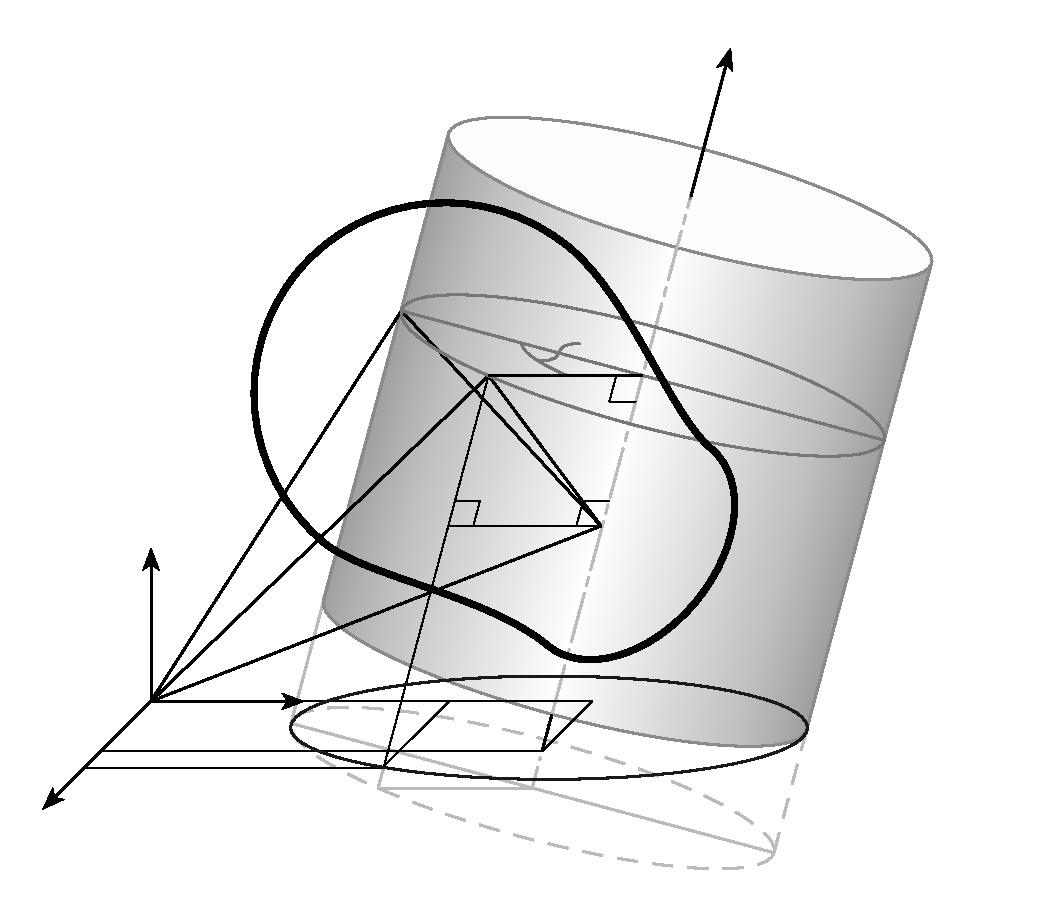
\includegraphics[width=\textwidth]{fig/rigid_rotation.pdf}
  \end{center}
  \caption{In reference frame $\cF$, 
  body $B$ rotating about axis $\vnhat$ an amount $\theta$, 
  which moves
  point $P$ in body $B$ to point $p$.}
  \label{fig:rigid_rotation}
\end{figure}

\clearpage
\begin{Hexample}
{
% %\colorbox{hlightgray}{Here we present a small example of artificially}
To come: nonlinear rigid pendulum.
% 
The governing nonlinear ordinary differential equation of motion,
\be
\ddot{\theta} + \frac{3 g}{2 L} \sin \theta = 0
\ee
% 
}
\end{Hexample}


\clearpage
\subsection{Isochoric (Poisson Special Case) Stretch}
Next consider a slightly different form of $\tFbold$, such that
\be
 \tFbold 
 = 
 \left[
 \begin{tabular}{cc}
  $\lambda$ & 0 \\
  0 & $\dst\frac{1}{\lambda}$
 \end{tabular}
 \right].
\ee
We keep the translation as $\vu = \vzero$.

For concreteness, consider $\lambda_1 = 2$ (expansion)
and $\lambda_2 = \half$ (contraction), as shown
in Fig.~\ref{fig:configuration_stretch}.

\begin{figure}[htb]
  \begin{center}
    %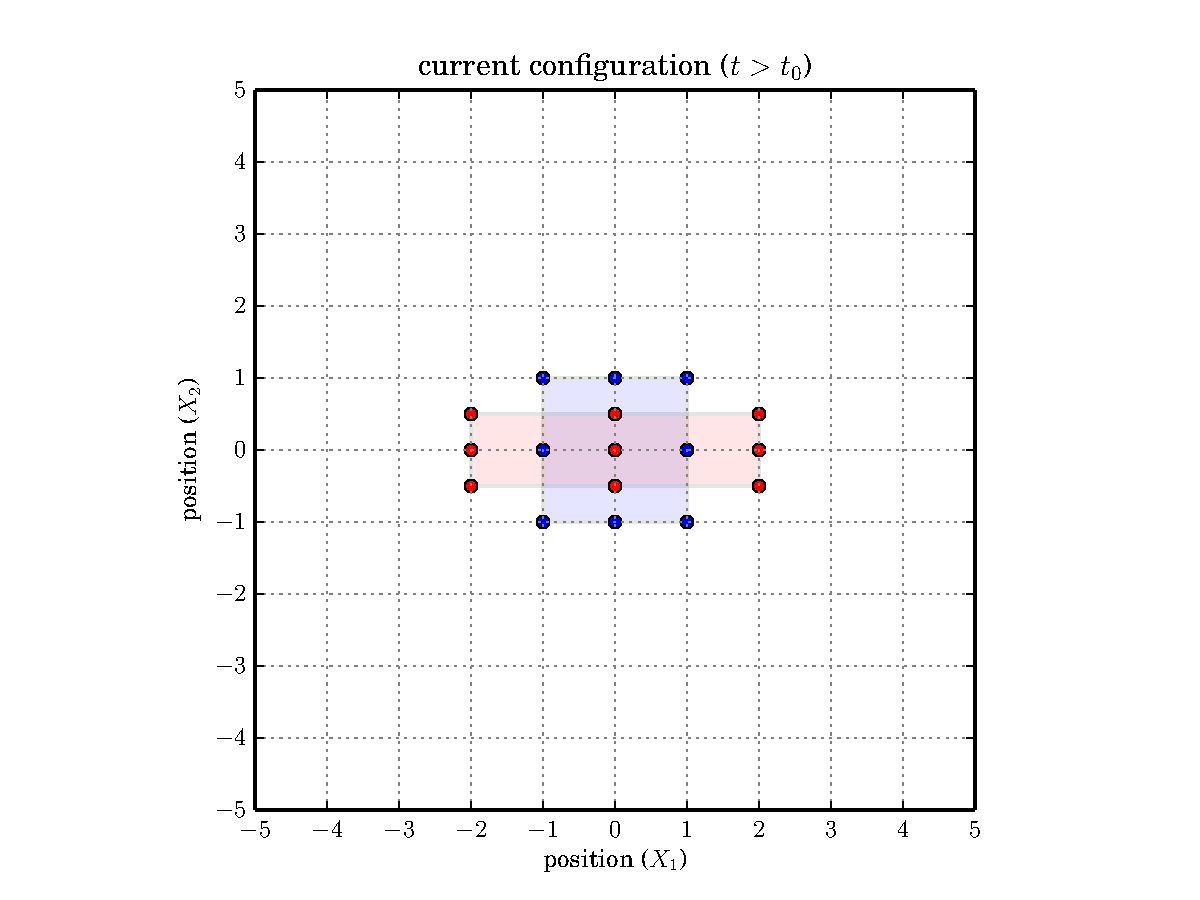
\includegraphics[width=\textwidth,natwidth=576,natheight=432]{fig/configuration_stretch.pdf}
    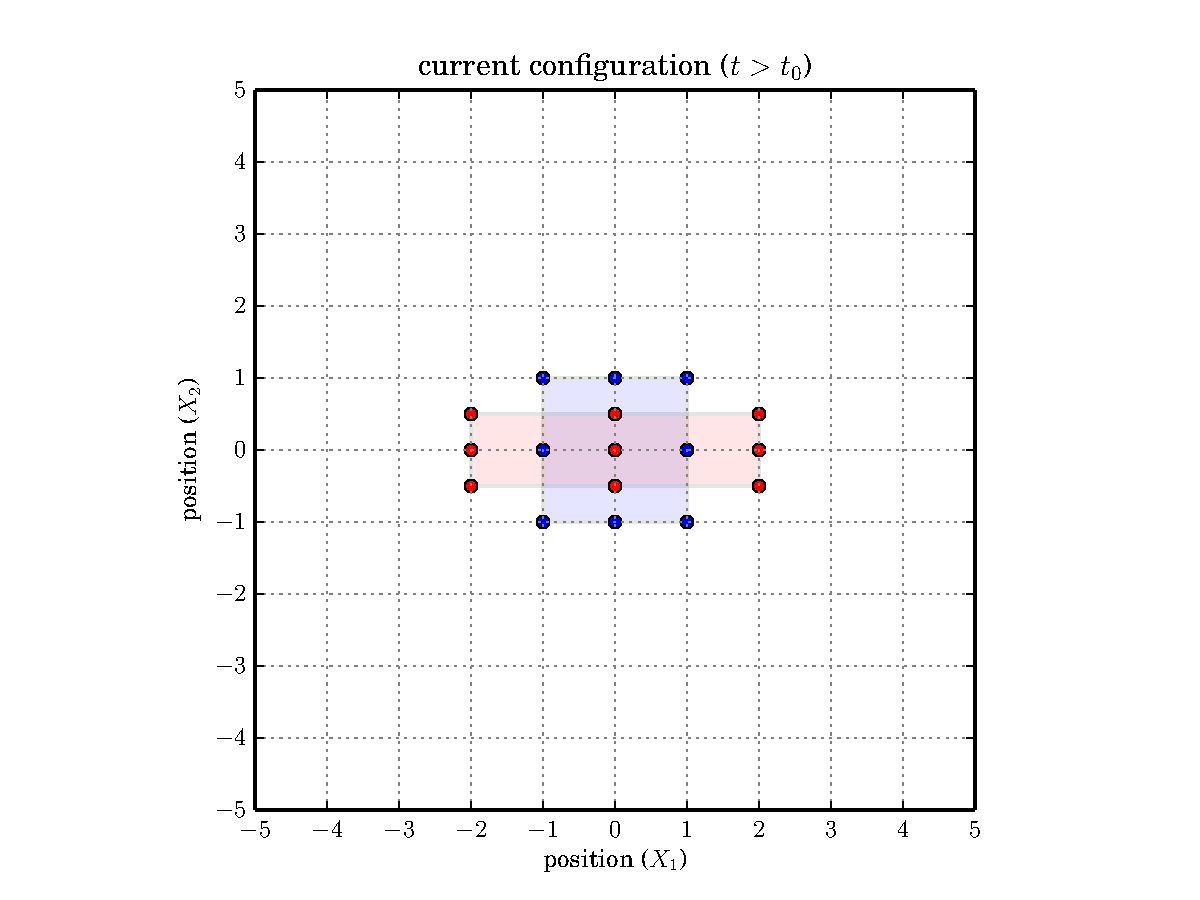
\includegraphics[width=\textwidth]{fig/configuration_stretch.pdf}
  \end{center}
  \caption{Illustration of an isochoric (deviatoric) motion.}
  \label{fig:configuration_stretch}
\end{figure}

The area in the reference configuration is $2 \times 2 = 4$, 
whereas the area in the current configuration is $4 \times 1 = 4$.   
For the sake of illustration, we have chosen stretches along the 
two axes such that the area does not change although the dimensions
and thus shape have changed.  This is an example of an 
{\bf isochoric} motion.  The roots {\em iso- (equal)} and {\em choro- (space)} 
describe a process from initial state $0$ to final state $1$
where the volume remains constant.  

In three dimensions, this case becomes
\be
 \tFbold 
 = 
 \left[
 \begin{tabular}{ccc}
  $\lambda_1$ & 0 & 0 \\
  0 & $\dst\frac{1}{\sqrt{\lambda}}$ & 0 \\
  0 & 0 & $\dst\frac{1}{\sqrt{\lambda}}$
 \end{tabular}
 \right].
\ee

Now, the motion as we have described it, doesn't yet show the {\em path}
taken between the reference and current configuration.  To 
get that detail, we would need to introduce the time parameter $t$, 
which we have suppressed for now.  
However, if we were to say the time interval is simply two points 
$t_0$ and $t_1$, we can create the path between these
two states $0$ and $1$, and connect with the isochoric process
$PV$ diagram in thermodynamics, shown in Fig.~\ref{fig:PV_isochoric}.

\begin{figure}[htb]
  \begin{center}
    %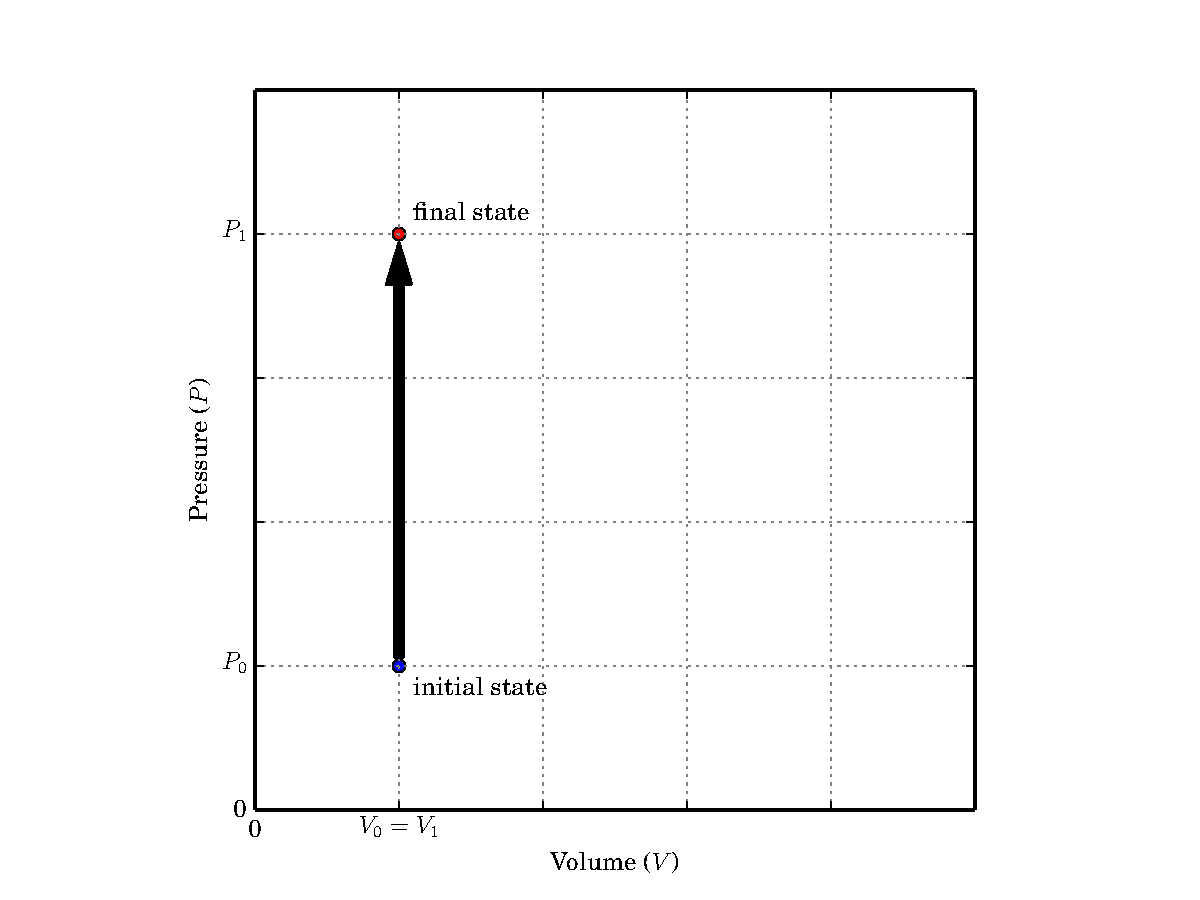
\includegraphics[width=\textwidth,natwidth=576,natheight=432]{fig/PV_isochoric.pdf}
    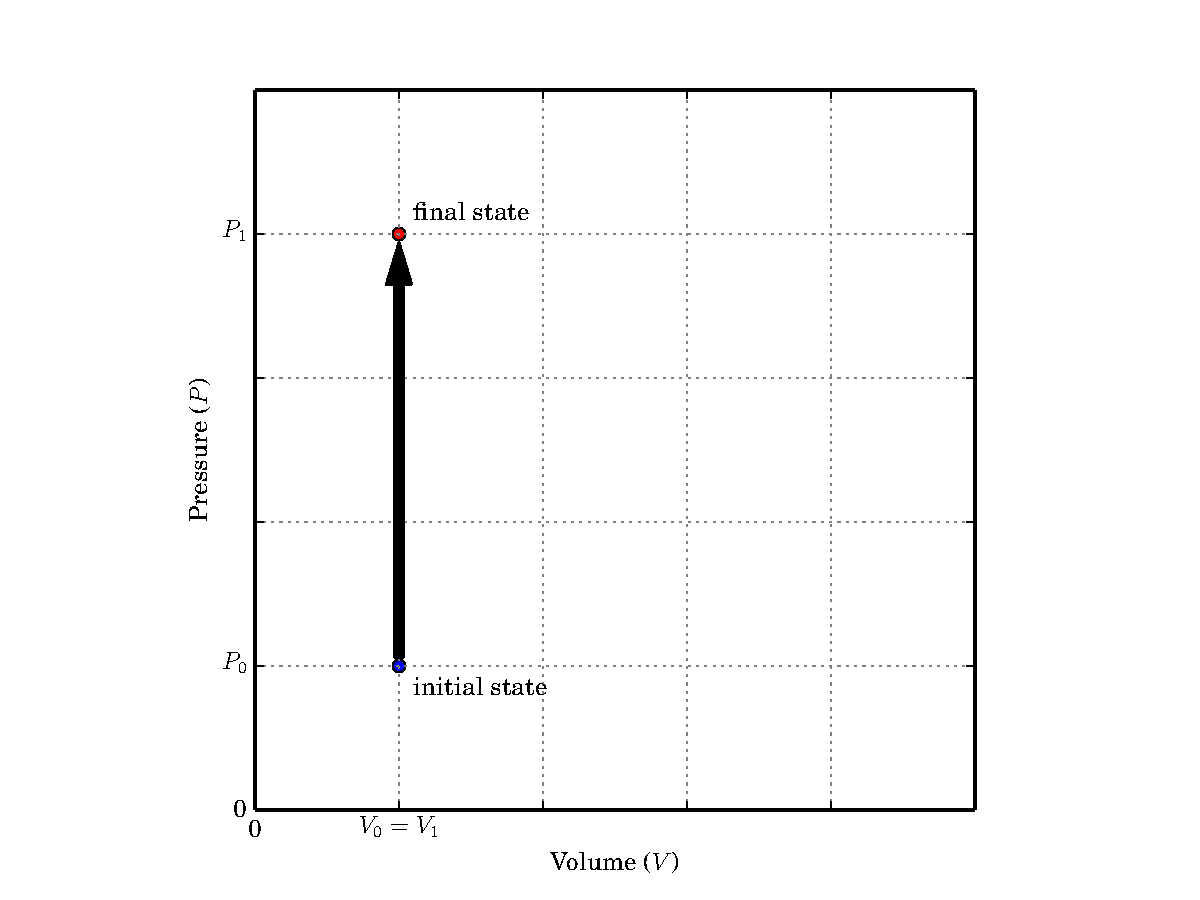
\includegraphics[width=\textwidth]{fig/PV_isochoric.pdf}
  \end{center}
  \caption{Isochoric process from initial state (reference configuration) $0$ to
  final state (current configuration) $1$.}
  \label{fig:PV_isochoric}
\end{figure}

We have yet to introduce and define pressure $P$, so this 
connection may be tenuous at the moment.  Nonetheless, we
introduce this connection now to motivate the single idea that
isochoric motions will play an important role in our later work.



\subsection{Dilatational (Volumetric) Stretch}
Consider now $\tFbold = \lambda \vid$ and $\vu = \vzero$.  
This describes {\bf volumetric} response, also known 
as a {\bf dilatational} response.  The parameter $\lambda \in \realplus$
causes the current configuration to change volume as
\begin{itemize}[noitemsep]
 \item $\lambda > 1$ expansion,
 \item $\lambda = 1$ identity,
 \item $0 < \lambda < 1$ contraction.
\end{itemize}
Notice that $\lambda$ describes the ``slope'' of the mapping from
reference to current configurations.  
In the case that $\lambda \rightarrow +\infty$, the volume grows infinite.  
In the case that $\lambda \rightarrow 0$, the volume shrinks to zero.
For concreteness, consider $\lambda = 2$.  The volumetric expansion
is shown in Fig.~\ref{fig:configuration_volumetric}.
The reference configuration, shown in blue, has area of~4.
The current configuration, shown in red, has area of~16.

\begin{figure}[htb]
  \begin{center}
    %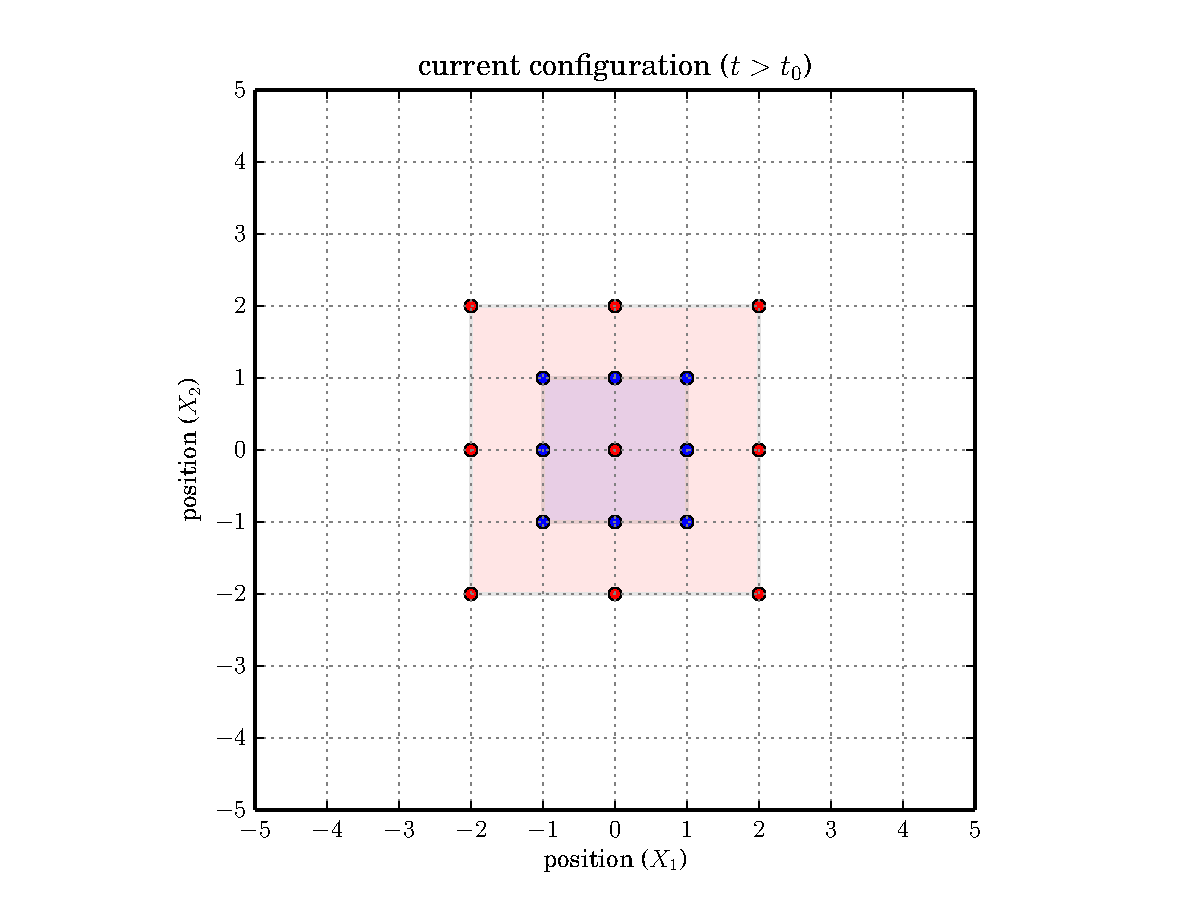
\includegraphics[width=0.9\textwidth,natwidth=576,natheight=432]{fig/configuration_volumetric.pdf}
    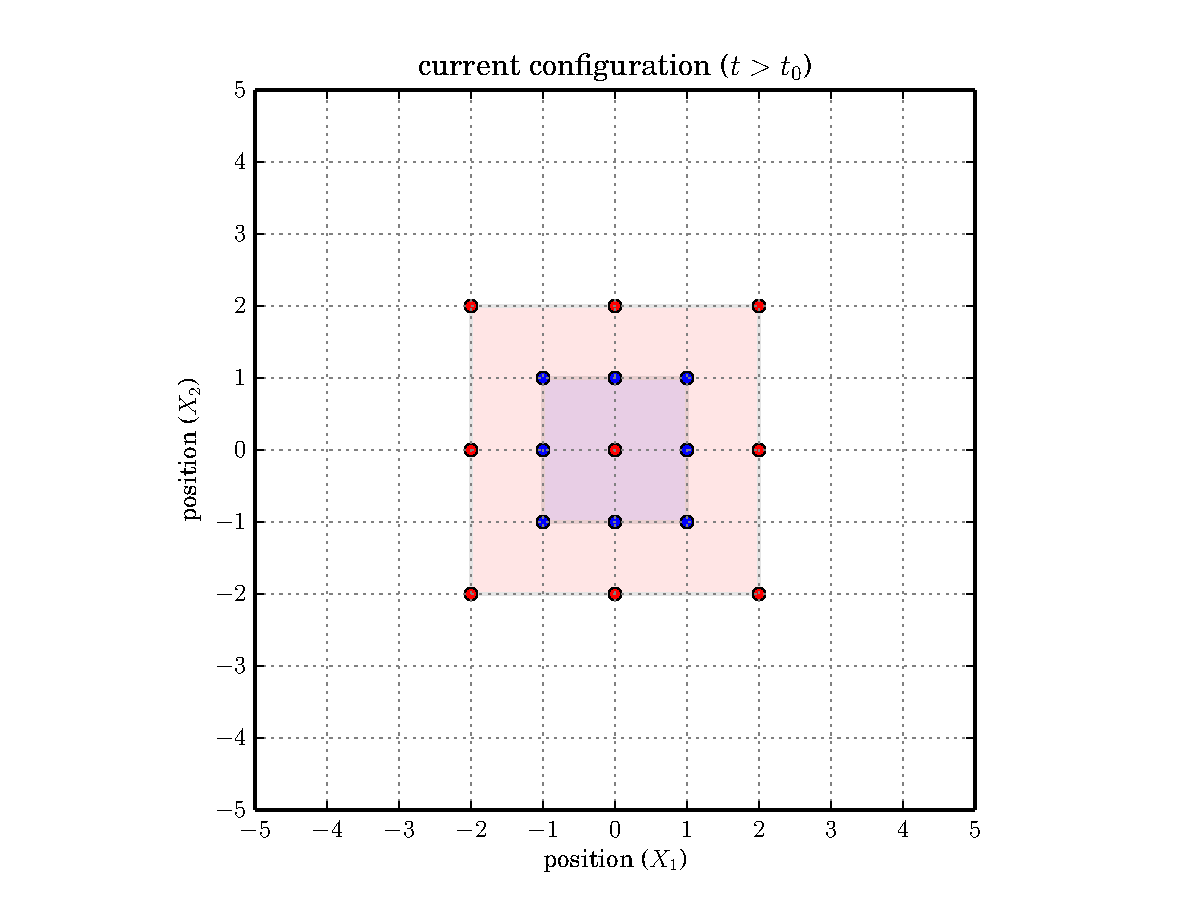
\includegraphics[width=0.9\textwidth]{fig/configuration_volumetric.pdf}
  \end{center}
  \caption{Illustration of a dilatational (volumetric) motion.}
  \label{fig:configuration_volumetric}
\end{figure}




\section{Rates}

\subsubsection{Total Time Derivative}
Let $\phi(\vx,t)$ be an arbitrary spatial scalar field and
let $\vphi(\vx,t)$ be an arbitrary spatial vector field.
For a body with spatial velocity $\vv(\vx, t)$, the total
time derivative of the scalar field $\phi$ is given by
\be
\boxed{
 \dot{\phi}(\vx, t) =
 \phi_{,t} 
  + \grad \phi 
 \cdot \vv
\;\; \Longleftrightarrow \;\;
 \dot{\phi} =  
 \frac{\partial \phi}{\partial t} 
 + 
 \frac{\partial \phi}{\partial x_i} \frac{\partial x_i}{\partial t}.
}
 \label{eq:total_time_derivative_scalar}
\ee
The total time derivate of the vector field $\vphi$ is given by
\be
\boxed{
 \dot{\vphi}(\vx, t) = 
 \vphi_{,t} 
 + [\grad \vphi] \; \vv
\;\; \Longleftrightarrow \;\;
 \dot{\phi}_i 
 = 
 \frac{\partial \phi_i}{\partial t} 
 + 
 \frac{\partial \phi_i}{\partial x_j} \frac{\partial x_j}{\partial t}.
 \label{eq:total_time_derivative_vector}
}
\ee
\begin{Hremark}
Some texts prefer the notation $\vv \cdot \grad \vphi$ to
$[\grad \vphi] \; \vv$, used in 
(\ref{eq:total_time_derivative_vector}).
\end{Hremark}


